\documentclass[]{beamer}
\usepackage[T1]{fontenc}
\usepackage[utf8]{inputenc}
\usepackage{lmodern}
\usepackage[italian]{babel}
\usepackage{mathrsfs}
\usepackage{cancel}


\title{Quantità di moto}
\author{\texorpdfstring{Mattia Cozzi\newline\href{mailto:cozzimattia@gmail.com}{\texttt{cozzimattia@gmail.com}}}{Mattia Cozzi}}
\date{a.s.~2023/2024}

%\documentclass[handout]{beamer}     %usare questa classe per generare l'handout
%\usepackage{pgfpages}   %per mostrare più quadri nella stessa pagina
%\pgfpagesuselayout{4 on 1}[a4paper,border shrink=5mm,landscape]
\usetheme{Singapore}
%\useoutertheme[left]{sidebar} %elementi intorno alle diapositive
\setbeamercovered{dynamic} %modifica l'aspetto del testo grigetto delle diapositive future. Argomenti: invisible/transparent/dynamic
\usecolortheme{orchid}
%COLORE PRINCIPALE
% \definecolor{marroncino}{RGB}{156, 26, 0} % UBC Blue (primary)
% \setbeamercolor{structure}{fg=marroncino} % itemize, enumerate, etc

\theoremstyle{plain}
\newtheorem{teorema}{Teorema}

\usepackage{tikz}
\usepackage{circuitikz}

\usepackage{pgf,pgfplots,graphicx}
\usetikzlibrary{angles,quotes,arrows,shapes,decorations.markings}
\pgfplotsset{compat=1.15}
\usepgfplotslibrary{units,fillbetween} % to add units easily to axis

\newcommand{\fem}{f_{em}}

\def\angolo[#1](#2)(#3:#4:#5)% Syntax: [draw options] (center) (initial angle:final angle:radius)
    { \draw[#1] ($(#2)+({#5*cos(#3)},{#5*sin(#3)})$) arc (#3:#4:#5); }


\newcommand<>{\xxcancel}[1]{\alt#2{\xcancel{#1}\vphantom{#1}}{#1}}

\begin{document}

\begin{frame}
  \titlepage
\end{frame}





\begin{frame}
\frametitle{Contenuti}
\tableofcontents
\end{frame}


\section{Quantità di moto}








\begin{frame}
\frametitle{Fenomeni}
\begin{columns}
\begin{column}{0.3\textwidth}
\visible<1->{\begin{figure}
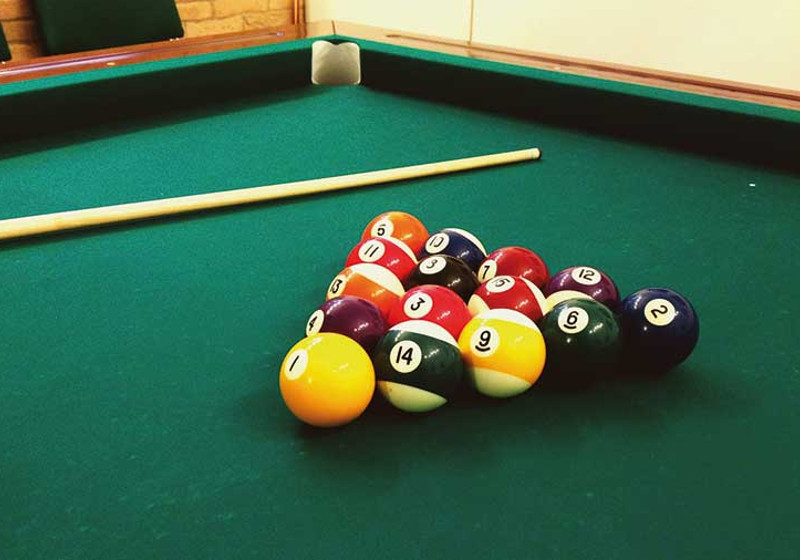
\includegraphics[width=\columnwidth]{img/biliardo.jpg}
\end{figure}}
\end{column}
\begin{column}{0.3\textwidth}
\visible<2->{\begin{figure}
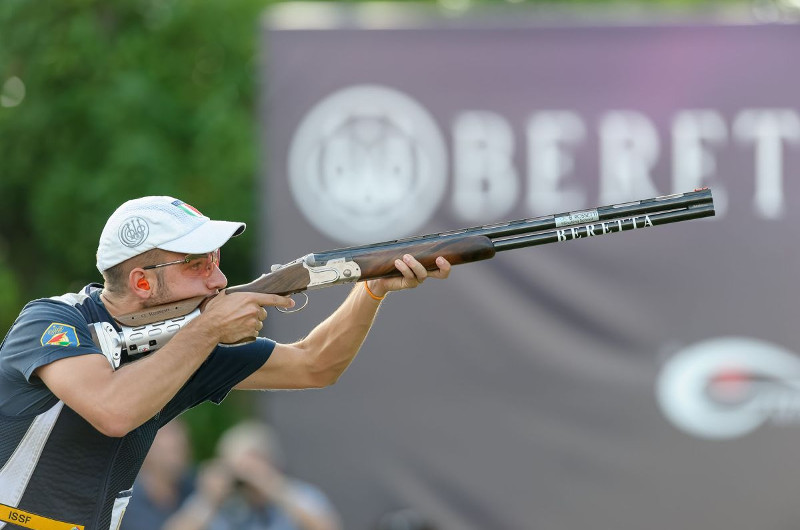
\includegraphics[width=\columnwidth]{img/tiroavolo.jpg}
\end{figure}}
\end{column}
\begin{column}{0.3\textwidth}
\visible<3->{\begin{figure}
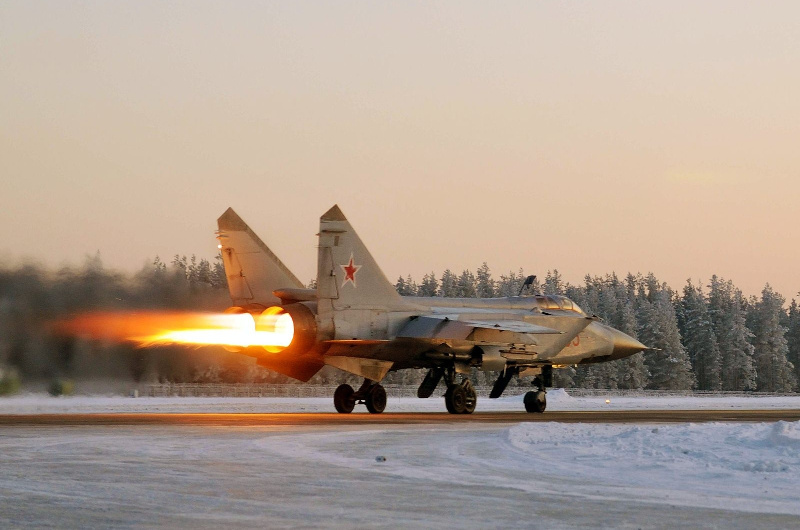
\includegraphics[width=\columnwidth]{img/aereoreazione.jpg}
\end{figure}}
\end{column}
\end{columns}

~

~

\visible<4->{Tutti questi fenomeni possono essere spiegati facendo riferimento ad una specifica \alert{legge di conservazione}.}
\end{frame}


\begin{frame}
\frametitle{Quantità di moto}
\begin{block}{Definizione}
La \emph{quantità di moto} di un corpo è il prodotto tra la sua massa e la sua velocità.

\begin{center}
\colorbox{blue!30}{$ \vec{p} = m\vec{v} $}~~~~~~~$ \left[ kg \cdot \frac{m}{s} \right] $
\end{center}
\end{block}\pause

~

Notiamo che la quantità di moto:
\begin{itemize}
  \item è definita come il prodotto tra uno scalare ed un vettore e pertanto \alert<2>{è una quantità vettoriale};\pause
  \item ha la \alert<3->{stessa direzione e verso di $ \vec{v} $}.
\end{itemize}
\end{frame}

\section{Conservazione}

\begin{frame}
\frametitle{Conservazione}
Per la quantità di moto vale il principio di:
\begin{block}{Conservazione della quantità di moto}
Se un sistema è isolato (cioè su di esso non agiscono forze esterne) la quantità di moto totale del sistema si conserva.

\begin{center}
\colorbox{blue!30}{$ \vec{p}_{tot_{iniziale}} = \vec{p}_{tot_{finale}} $}
\end{center}
\end{block}\pause

~

Questo principio di conservazione è una conseguenza dei principi della dinamica, da cui parte la dimostrazione.
\end{frame}



\begin{frame}
\frametitle{Dimostrazione della conservazione}
Supponiamo che due corpi $ A $ e $ B $ si urtino, esercitando una forza l'uno sull'altro per un tempo $ \Delta t $:
\begin{center}
$ \vec{F}_{A\, su\, B} = - \vec{F}_{B\, su\, A} $~~~(TPD) \pause

~

$ m_A \vec{a}_A = - m_B \vec{a}_B $~~~(SPD)\pause

~

$ m_A \dfrac{\Delta \vec v_A}{\xxcancel<4->{\Delta t}} = - m_B \dfrac{\Delta \vec v_B}{\xxcancel<4->{\Delta t}} $\pause

~

$ m_A (\vec{v}_{A_{fin}} - \vec{v}_{A_{ini}}) = - m_B (\vec{v}_{B_{fin}} - \vec{v}_{B_{ini}}) $\pause

~

$ m_A \vec{v}_{A_{fin}} + m_B \vec{v}_{B_{fin}} = m_A \vec{v}_{A_{ini}} + m_B \vec{v}_{B_{ini}} $\pause


~

$ \vec{p}_{A_{fin}} + \vec{p}_{B_{fin}} = \vec{p}_{A_{ini}} + \vec{p}_{B_{ini}} $\pause

~

\colorbox{blue!30}{$ \vec{p}_{tot_{fin}} = \vec{p}_{tot_{ini}} $}
\end{center}
\end{frame}




\begin{frame}
\frametitle{Esempio 1}
\begin{exampleblock}{Lancio di un oggetto da un corpo libero}
{\small Un bambino di massa $ m_B = 30,0 \, kg $ tiene in mano una palla di massa $ m_P = 3,00 \, kg $. Il bambino è fermo su uno skateboard senza attrito. Ad un certo punto il ragazzo lancia orizzontalmente la palla con velocità $ v_P = 8,00 \, \frac{m}{s} $. 

A che velocità si muove il bambino dopo il lancio?}
\end{exampleblock}\pause

~

Poiché inizialmente  il sistema palla-bambino è fermo, la quantità di moto iniziale è nulla.{\pause} Così dovrà essere anche dopo il lancio, e quindi:
\begin{center}
$ \vec{p}_P + \vec{p}_B = 0 $
\end{center}
\end{frame}


\begin{frame}
\frametitle{Esempio 1}
Passiamo ai moduli, in quanto i due vettori sono paralleli:
\begin{center}
$ p_B + p_P = 0 $\pause

~

$ p_B = - p_P $\pause

~

$ m_B v_B = - m_P v_P $\pause

~

$ v_B = - \dfrac{m_P}{m_B} v_P $\pause

~

$ v_B = - \dfrac{3,00 \, \cancel{kg}}{30,0 \, \cancel{kg}} \cdot 8,00 \, \frac{m}{s} = - 0,10 \cdot 8,00 \, \frac{m}{s} = - 0,80 \, \frac{m}{s} $
\end{center}\pause
Notiamo che, avendo una massa dieci volte superiore alla palla, il bambino si muoverà al $ 10\% $ della velocità della palla.
\end{frame}



\section{Impulso}

\begin{frame}
\frametitle{Teorema dell'impulso}
Riformuliamo il secondo principio della dinamica:
\begin{center}
$ \vec{F} = m \vec{a} $\pause

~

$ \vec{F} = m \dfrac{\Delta \vec{v}}{\Delta t}  $\pause

~

$ \vec{F}\Delta t = m \Delta\vec{v} $\pause

~

\colorbox{blue!30}{$ \vec{F}\Delta t = \Delta\vec{p} $}\pause
\end{center}
\alert<5>{Se una forza $ \vec{F} $ agisce su un corpo per un tempo $ \Delta t $ ne causa una variazione di quantità di moto $ \Delta \vec{p} $}.\pause

~

Tale variazione è detta \alert<6>{impulso della forza: $ \vec{I} = \Delta \vec{p} $}.
\end{frame}


\begin{frame}
\frametitle{Lavoro e impulso}

\begin{columns}
\begin{column}{0.5\textwidth}
\begin{center}
\colorbox{blue!30}{$ L = \vec{F} \cdot \alert<1->{\Delta\vec{s}} $}
\end{center}
\visible<1->{Il lavoro descrive l'effetto di una forza che agisce per una certa \alert<1->{distanza}.}
\end{column}
\begin{column}{0.5\textwidth}
\visible<2->{\begin{center}
\colorbox{blue!30}{$ \vec{I} = \vec{F} \alert<2>{\Delta t} $}
\end{center}
L'impulso descrive l'effetto di una forza che agisce per un certo \alert<2->{tempo}.}
\end{column}
\end{columns}
\end{frame}






\begin{frame}
\frametitle{Esempio 2}
\begin{exampleblock}{Velocità finale}
{\small Un oggetto di massa $ m=2,0 \, kg $ è in moto a velocità costante $ v_0 = 4,5 \, \frac{m}{s} $. Subisce poi una forza di $ 17 \, N $ per un tempo di $ 3,0 \, s $.
\begin{itemize}
  \item Quanto vale la velocità finale $ v_1 $ dell'oggetto?
\end{itemize}}
\end{exampleblock}\pause

~


Scopriremo la variazione di velocità a partire dalla variazione di quantità di moto:
\begin{center}
$ F\Delta t = \Delta p $\pause

~

$ F \Delta t = mv_1 - mv_0 $\pause

~

$ F\Delta t + mv_0 = mv_1 $ 
\end{center}
\end{frame}


\begin{frame}
\frametitle{Esempio 2}
\begin{center}
$ \dfrac{F\Delta t}{m} + v_0 = v_1 $\pause

~

~

$ v_1 = \dfrac{17 \, N \cdot 3,0 \, s}{2,0 \, kg} + 4,5 \, \frac{m}{s} $

~

~

$\pause v_1 = 25,5 \, \frac{m}{s} + 4,5 \, \frac{m}{s} = 30 \, \frac{m}{s} $\end{center}
\end{frame}








\section{Urti}



\begin{frame}
\frametitle{Urti nel piano}
\begin{figure}
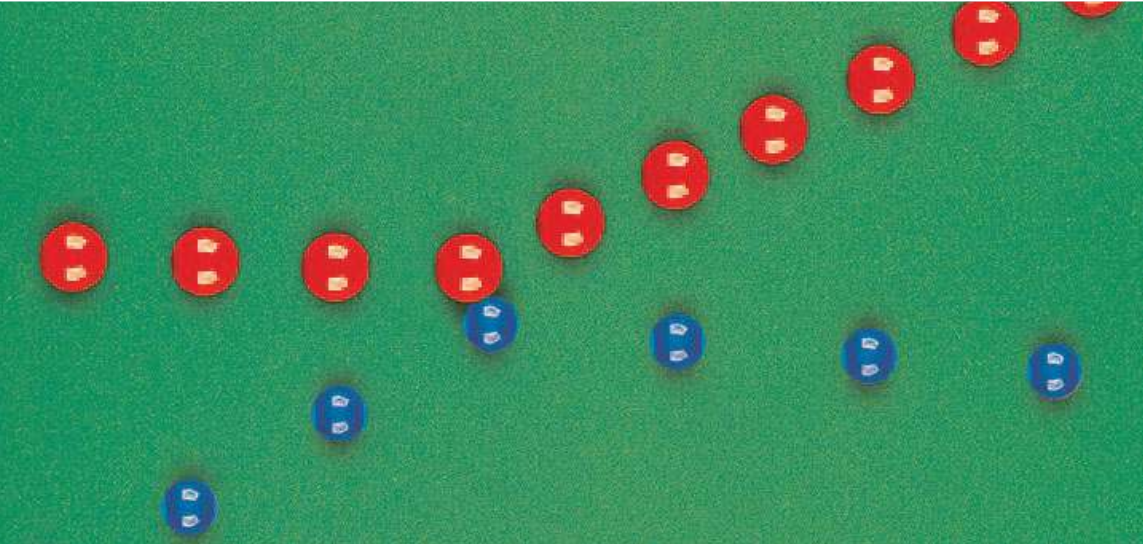
\includegraphics[width=.6\columnwidth]{img/biglie.png}
\end{figure}
\visible<2->{
\begin{figure}
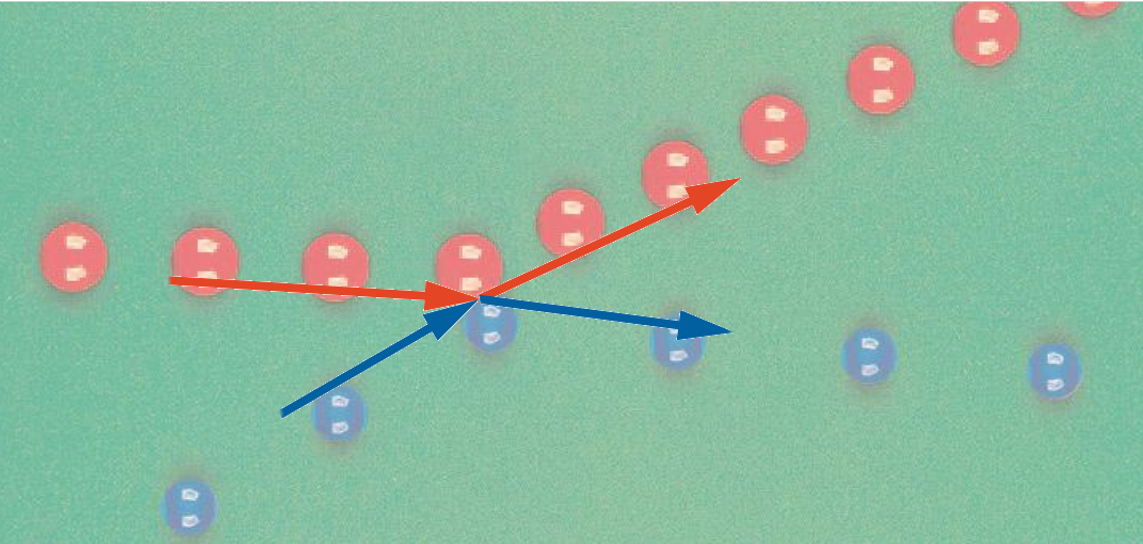
\includegraphics[width=.6\columnwidth]{img/biglie2.png}
\end{figure}}
\end{frame}




\begin{frame}
\frametitle{Analisi vettoriale}
\begin{figure}
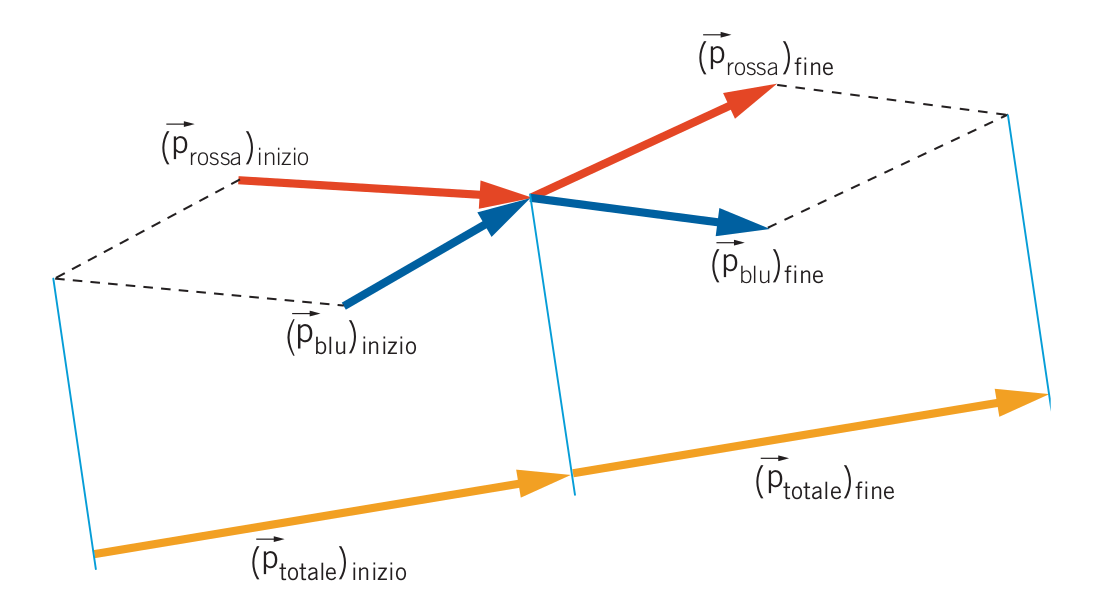
\includegraphics[width=.8\columnwidth]{img/urto2d.png}
\end{figure}
\end{frame}




\begin{frame}
\frametitle{Urti su una retta (1)}
Analizziamo il caso di urti che avvengono su una retta.\pause

~

Valgono le seguenti considerazioni:
\begin{itemize}
  \item durante un urto i due corpi si comportano come un \alert<2>{sistema isolato};\pause
  \item dal punto sopra, la \alert<3>{quantità di moto totale si conserva};\pause
  \item possiamo ridurre le somme tra vettori a \alert<4>{somme algebriche}, poiché lavoriamo in una dimensione sola.
\end{itemize}
\end{frame}

\begin{frame}
\frametitle{Urti su una retta (2)}
\begin{figure}
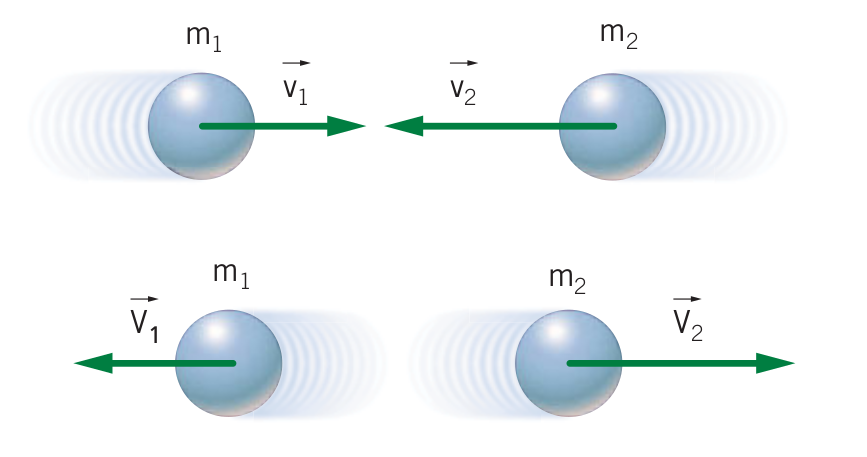
\includegraphics[width=.5\columnwidth]{img/urto1d.png}

~


$ m_1 v_1 + m_2 v_2 = m_1 V_1 + m_2 V_2 $
\end{figure}
\end{frame}



\begin{frame}
\frametitle{Urto elastico e urto anelastico}
Distinguiamo tre tipi di urto:
\begin{itemize}
  \item \alert<1>{urto elastico}, in cui i corpi si comportano come molle che si deformano senza dissipare energia cinetica;\pause
  \item \alert<2>{urto anelastico}, in cui i corpi si deformano e nel farlo assorbono una parte dell'energia cinetica;\pause
  \item \alert<3>{urto completamente anelastico}, in cui i corpi restano uniti dopo l'urto.
\end{itemize}
\end{frame}

\begin{frame}
\frametitle{Urto elastico}
Se l'urto è elastico avremo il sistema:
\[
\left\{ 
\begin{array}{l}
p_{tot_{iniziale}} = p_{tot_{finale}}\\
~\\
K_{tot_{iniziale}} = K_{tot_{finale}}
\end{array}
\right. 
\]\pause

~

Si risolve come un qualsiasi sistema di due equazioni a due incognite.
\end{frame}






\begin{frame}
\frametitle{Esempio 3}
\begin{exampleblock}{Urto elastico tra carrelli}
{\small Due carrelli si muovono su un binario rettilineo e si urtano in modo elastico. Prima dell'urto uno di essi, che ha una massa di $ 2,0 \, kg $, si muoveva verso destra con una velocità di $ 5,0 \, \frac{m}{s} $, mentre il secondo (la cui massa è $ 1,0 \, kg $) si spostava verso sinistra a $ 4,0 \, \frac{m}{s} $.
\begin{itemize}
  \item Quali sono le velocità dei due carrelli dopo l'urto?
\end{itemize}}
\end{exampleblock}
\end{frame}




\begin{frame}
\frametitle{Urto completamente anelastico}

Se l'urto è completamente anelastico la velocità finale $ V $ dei due corpi sarà determinata unicamente dalla quantità di moto:
\begin{center}
$ m_1 v_1 + m_2 v_2 = (m_1 + m_2) V ~~~~\Longrightarrow~~~~  V = \dfrac{m_1 v_1 + m_2 v_2}{m_1 + m_2} $
\end{center}
\end{frame}




\section{Centro di massa}







\begin{frame}
\frametitle{Il centro di massa}
Per corpi estesi (cioè non riducibili a punti materiali) e sistemi di particelle, possiamo individuare un punto particolare, il \alert<1>{centro di massa} (baricentro).\pause

~

Il centro di massa ha una proprietà fondamentale:
\begin{block}{Moto del centro di massa}
  Quando un corpo esteso o un sistema si muove per inerzia o subisce una forza, \alert<2>{il centro di massa si muove come un punto materiale}.
\end{block}\pause

~

Possiamo quindi riportare lo studio del moto dei corpi estesi a quanto già noto per i punti materiali.
\end{frame}


\begin{frame}
\frametitle{Moto del centro di massa}
\begin{figure}
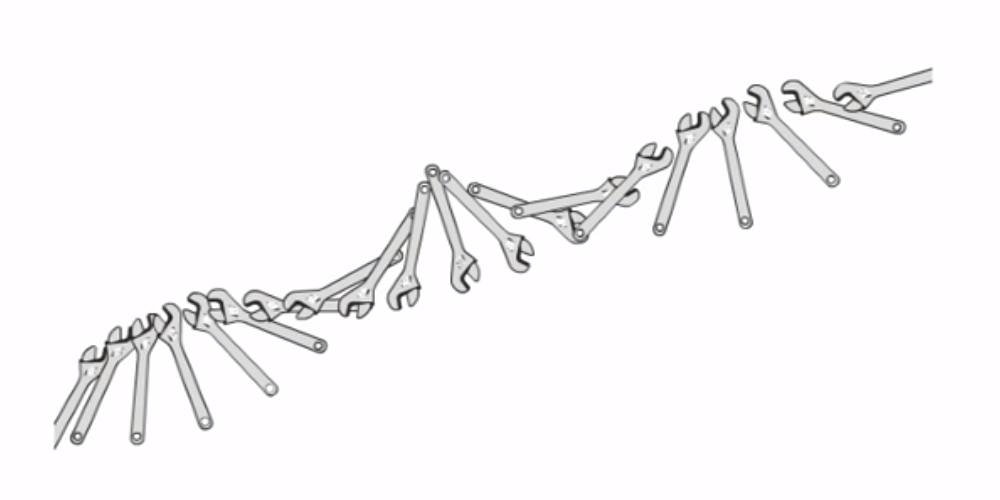
\includegraphics[width=.6\columnwidth]{img/cdm1.png}

\visible<2->{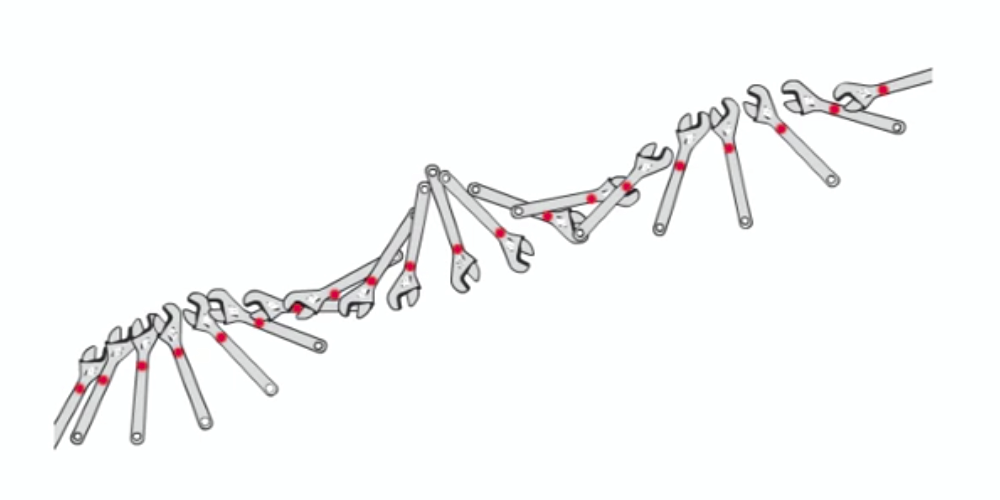
\includegraphics[width=.6\columnwidth]{img/cdm2.png}}

\visible<0>{\href{video/Centrodimassa.mp4}{\beamergotobutton{Video: Moto del cdm di oggetti sottoposti alla forza peso}}}
\end{figure}
\end{frame}

\begin{frame}
\frametitle{Moto del centro di massa}
\begin{figure}
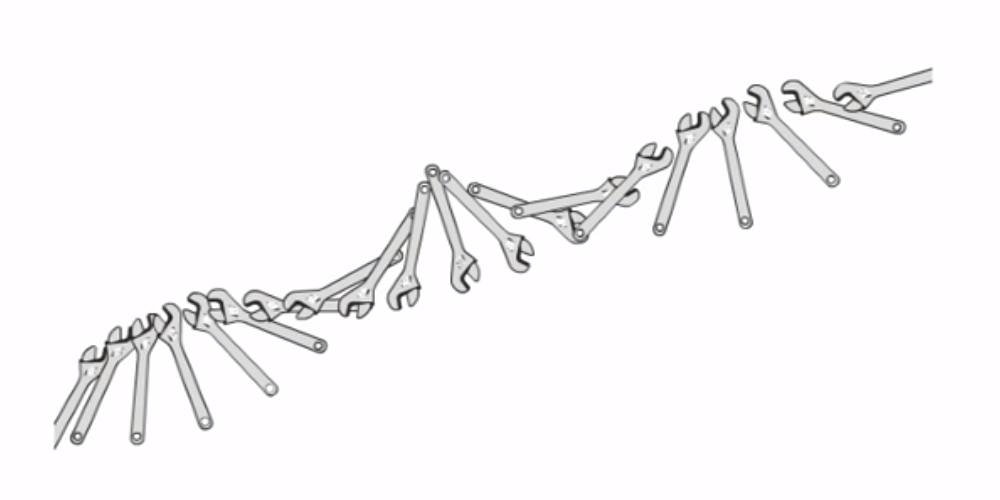
\includegraphics[width=.6\columnwidth]{img/cdm1.png}

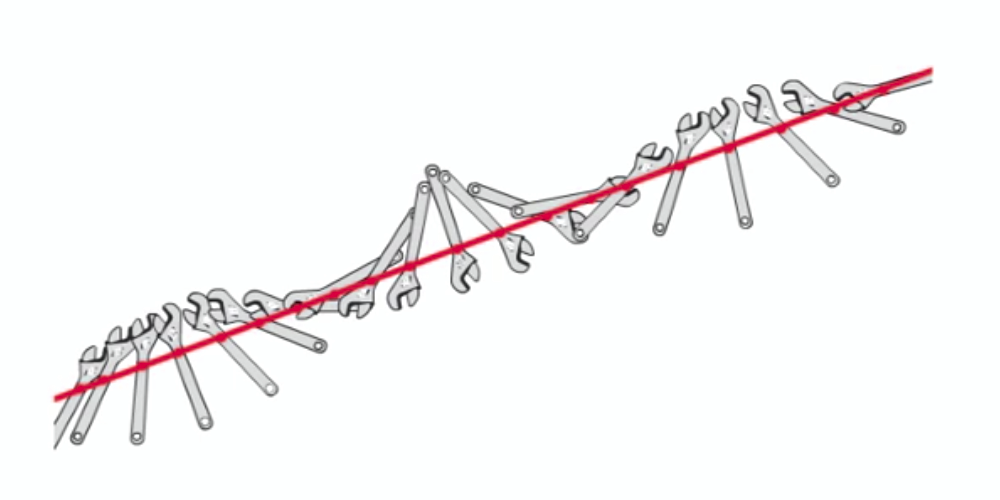
\includegraphics[width=.6\columnwidth]{img/cdm3.png}

\href{video/Centrodimassa.mp4}{\beamergotobutton{Video: Moto del cdm di oggetti sottoposti alla forza peso}}
\end{figure}
\end{frame}


\begin{frame}
\frametitle{Posizione del centro di massa}
Se $ m_1 $, $ m_2 $,..., $ m_n $ sono le masse del sistema poste nelle posizioni $ x_1 $, $ x_2 $,..., $ x_n $, allora l'ascissa del centro di massa sarà:
\begin{center}
$ x_{cdm} = \dfrac{m_1 x_1 + m_2 x_2 + ... + m_n x_n}{m_1 + m_2 + ... + m_n} $
\end{center}
Similmente si procede per l'ordinata.\pause

~

Notiamo che il centro di massa è definito dalla \emph{media pesata} della distanza delle particelle da un punto.
\end{frame}





\begin{frame}
\frametitle{Esempio 4}
\begin{exampleblock}{Posizione del centro di massa}
{\small La massa del Sole è $ 2,0 \times 10^{30} \, kg $ e quella della Terra è $ 6,0 \times 10^{24} \, kg $. La distanza Terra-Sole vale $ 1,5 \times 10^{11} \, m $. Fissa nel centro del Sole l'origine del sistema di coordinate.
\begin{itemize}
  \item Dove si trova il centro di massa del sistema Terra-Sole?
\end{itemize}}
\end{exampleblock}\pause

~

Chiamiamo $ x $ la posizione del centro di massa e rappresentiamo:
\begin{figure}
\begin{tikzpicture}[scale=.5]
\draw [dashed] (0,0) --(8,0);
\draw [] (2,-.2) --(2,.2);
\draw [red,thick,fill=orange] (0,0) circle [radius=0.4];
\draw [green,thick,fill=cyan] (8,0) circle [radius=0.15];
\node [above] at (8,.2) {\footnotesize$ d $};
\node [above] at (2,.2) {\footnotesize$ x $};
\node [below left] at (-.1,-.1) {\footnotesize$ M $};
\node [below right] at (8.1,-.1) {\footnotesize$ m $};
\end{tikzpicture}
\end{figure}
\end{frame}


\begin{frame}
\frametitle{Esempio 4}
\begin{figure}
\begin{tikzpicture}[scale=.5]
\draw [dashed] (0,0) --(8,0);
\draw [] (2,-.2) --(2,.2);
\draw [red,thick,fill=orange] (0,0) circle [radius=0.4];
\draw [green,thick,fill=cyan] (8,0) circle [radius=0.15];
\node [above] at (8,.2) {\footnotesize$ d $};
\node [above] at (2,.2) {\footnotesize$ x $};
\node [below left] at (-.1,-.1) {\footnotesize$ M $};
\node [below right] at (8.1,-.1) {\footnotesize$ m $};
\end{tikzpicture}
\end{figure}
\begin{center}
$ x = \dfrac{M \cdot 0 + m \cdot d}{M+m} $\pause

~

~

$ x = \dfrac{m}{M+m}d = \pause 4,5 \times 10^{5} \, m $
\end{center}
\end{frame}




\end{document}
